%%%%%%%%%%%%%%%%%%%%%%%%%%%%%%%%%%%%%%%%%%%%%%%%%%%%%%%%%%%%%%%%%%%%%%%%
%% Práctica de Métodos de Simulación (MUIA). Enunciado 9, Ejercicio 1.
%% Estilo adaptado de la plantilla oficial de la ETSI Informáticos (UPM),
%% versión 2023.06.01: A4, Bookman 11 pt, márgenes 3,5/3 cm, numeración
%% decimal y número de página centrado en el pie.
%% Compilar con: pdflatex memoria_ej1 (dos pasadas)
%%%%%%%%%%%%%%%%%%%%%%%%%%%%%%%%%%%%%%%%%%%%%%%%%%%%%%%%%%%%%%%%%%%%%%%%
\documentclass[a4paper,11pt]{article}

%% Configuración relacionada con normativa
\usepackage[T1]{fontenc}
\usepackage[utf8]{inputenc}
\usepackage[english,spanish,es-lcroman,es-noshorthands,es-tabla]{babel}
\usepackage[top=3.5cm,bottom=3.5cm,right=3cm,left=3cm]{geometry}
\usepackage{bookman}

%% Cabeceras y pies de página
\usepackage{fancyhdr}
\pagestyle{fancy}
\fancyhf{}
\fancyhead[R]{\small\textbf{\rightmark}}
\fancyhead[L]{\small Métodos de Simulación -- Ejercicio 1}
\setlength{\headheight}{1.5\headheight}
\cfoot{\thepage}
\renewcommand{\sectionmark}[1]{\markright{\thesection. #1}}

%% Paquetes
\usepackage{amsmath,amssymb}
\usepackage{graphicx}
\usepackage{float}
\usepackage{booktabs}
\usepackage{tabularx}
\usepackage{array}
\usepackage{parskip}
\usepackage{csquotes}
\usepackage{xcolor}
\usepackage{enumitem}
\usepackage[pdfborder={0 0 0},pdfusetitle]{hyperref}
\setlist{nosep,leftmargin=*}

%% Código (colores de la plantilla oficial)
\usepackage{listings}
\definecolor{commentcolor}{rgb}{.804,0,0}
\definecolor{keywordcolor}{rgb}{.608,.19,1}
\definecolor{stringcolor}{rgb}{0,.545,0}
\lstset{
  language=C,
  basicstyle=\ttfamily\footnotesize,
  commentstyle=\itshape\color{commentcolor},
  keywordstyle=\bfseries\color{keywordcolor},
  stringstyle=\color{stringcolor},
  frame=lines,
  framesep=4pt,
  breaklines=true,
  columns=fullflexible,
  keepspaces=true,
  showstringspaces=false,
  extendedchars=true,
  literate=
  {á}{{\'a}}1 {é}{{\'e}}1 {í}{{\'i}}1 {ó}{{\'o}}1 {ú}{{\'u}}1
  {Á}{{\'A}}1 {É}{{\'E}}1 {Í}{{\'I}}1 {Ó}{{\'O}}1 {Ú}{{\'U}}1
  {ñ}{{\~n}}1 {Ñ}{{\~N}}1 {ü}{{\"u}}1 {¿}{{?`}}1 {¡}{{!`}}1
}

%% Símbolos de resultado de Dieharder
\newcommand{\PA}{\textsf{P}}
\newcommand{\WK}{\textbf{\textsf{W}}}
\newcommand{\FA}{\textbf{\textsf{\color{commentcolor}F}}}

%% Datos del trabajo
\newcommand{\Estudios}{Máster Universitario}
\newcommand{\TituloEstudios}{Inteligencia Artificial}
\newcommand{\Asignatura}{Métodos de Simulación}
%% REVISAR: nombres completos de los miembros del grupo 9
\newcommand{\NombreAutor}{Eder Tarifa, Xi Xu, Luis Carles y Juan Rodríguez Díaz de Greñu}
\newcommand{\Profesores}{Antonio Jiménez Martín}
\newcommand{\TituloTrabajo}{Generación de Números Aleatorios con el Generador Congruencial de IMSL y Contrastes de Aleatoriedad Diehard}
\newcommand{\Fecha}{Noviembre 2026}
\title{\TituloTrabajo}
\author{\NombreAutor}
\date{\Fecha}

\usepackage{url}
\DeclareUrlCommand\code{\urlstyle{tt}}
\renewcommand{\UrlBreaks}{\do\:\do\/\do\_\do\#\do\.\do\-}
\setlength{\emergencystretch}{2em}

\begin{document}

%%%%%%%%%%%%%%%%%%%%%%%%%%%%%%%%%%%%%%%%%%%%%%%%%%%%%%%%%%%%%%%%%%%%%%%%
%% Portada (plantilla oficial de la ETSI Informáticos)
\begin{titlepage}
\begin{minipage}{0.15\linewidth}
\hspace*{-15mm}
\noindent

\includegraphics[scale=0.5]{portada/escudo_upm.png}
\end{minipage}
\begin{minipage}{0.7\linewidth}
\begin{center}
\huge{Universidad Politécnica\\de Madrid}\\
\vspace*{0.5cm}
\Large{\textbf{Escuela Técnica Superior de \\ Ingenieros Informáticos}}
\end{center}
\end{minipage}
\begin{minipage}{0.2\linewidth}

\includegraphics[scale=0.5]{portada/escudo_etsiinf.png}
\end{minipage}

\vspace*{1cm}
\begin{center}
\Large{\Estudios\ en \TituloEstudios}
\end{center}

\vspace*{1cm}
\begin{center}
\huge{\Asignatura}\\[0.3cm]
\Large{Práctica -- Enunciado 9 -- Ejercicio 1}
\end{center}

\vspace*{0.5cm}
\begin{center}
\huge\bfseries{\TituloTrabajo}
\end{center}

\vspace*{3cm}

\noindent
\large{Grupo 9}\\
\large{Autores: \NombreAutor}\\
\large{Profesor: \Profesores}

\vspace*{2.5cm}
\begin{center}
Madrid, \Fecha
\end{center}
\end{titlepage}

\tableofcontents
\newpage

%%%%%%%%%%%%%%%%%%%%%%%%%%%%%%%%%%%%%%%%%%%%%%%%%%%%%%%%%%%%%%%%%%%%%%%%
\section{Introducción}

El enunciado pide, utilizando el generador congruencial multiplicativo de la
librería IMSL
\begin{equation}\label{eq:lcg}
  x_{i+1} = 16807\, x_i \bmod (2^{31}-1),
\end{equation}
obtener una muestra de números aleatorios en $(0,1)$ y estudiar su
aleatoriedad con los contrastes de la librería \emph{Diehard}, explicando
brevemente en qué consisten tres de ellos.

Para ello se ha implementado el generador en C (sección~\ref{sec:generador}),
se ha validado frente al valor de control publicado por sus autores y se ha
sometido a dos bloques de contrastes (sección~\ref{sec:metodologia}): seis
contrastes clásicos del tema~2 de la asignatura y la batería Diehard completa,
ejecutada con \emph{Dieharder}~\cite{dieharder}, la reimplementación mantenida de
la batería original de Marsaglia~\cite{diehard}. Los resultados se presentan en
las secciones~\ref{sec:clasicos} y~\ref{sec:diehard}. La
sección~\ref{sec:tres} explica tres de los contrastes y la
sección~\ref{sec:conclusiones} resume las conclusiones.

%%%%%%%%%%%%%%%%%%%%%%%%%%%%%%%%%%%%%%%%%%%%%%%%%%%%%%%%%%%%%%%%%%%%%%%%
\section{El generador}\label{sec:generador}

\subsection{Definición y propiedades}

La expresión~\eqref{eq:lcg} es el generador \enquote{estándar mínimo}
propuesto por Lewis, Goodman y Miller en 1969 y defendido por Park y
Miller~\cite{parkmiller} como referencia mínima de calidad. Es el que usa la
rutina \code{RNUN} de IMSL en su opción por defecto. Sus parámetros son el
multiplicador $a = 16807 = 7^5$, el módulo $m = 2^{31}-1 = 2\,147\,483\,647$
(un primo de Mersenne) y el incremento $c = 0$.

\begin{itemize}
  \item \textbf{Periodo.} Al ser $m$ primo y $c=0$, el periodo máximo es $m-1$,
        y se alcanza si y solo si $a$ es raíz primitiva módulo $m$~\cite{riosinsua,knuth}.
        Como 7 es raíz primitiva de $m$ y $\gcd(5, m-1) = 1$, también lo es
        $7^5$. El periodo es, por tanto, $m-1 = 2^{31}-2 \approx 2{,}15\cdot10^{9}$
        para cualquier semilla $x_0 \in \{1,\dots,m-1\}$.
  \item \textbf{Rango.} Como $x_i \in \{1,\dots,m-1\}$, los valores
        $u_i = x_i/m$ nunca valen 0 ni 1. La muestra está contenida en $(0,1)$,
        como pide el enunciado.
  \item \textbf{Estructura en retículo.} Como todo generador congruencial, los
        vectores $(u_i, u_{i+1},\dots,u_{i+k-1})$ caen sobre un número reducido
        de hiperplanos paralelos (teorema de Marsaglia). Se observa en la
        figura~\ref{fig:pares}.
\end{itemize}

\subsection{Implementación}

El programa \code{lcg.c} implementa la recurrencia de dos formas: con
aritmética entera de 64 bits y con el método de Schrage, que evita el
desbordamiento usando solo enteros de 32 bits con signo. Para ello descompone
$m = aq + r$ con $q = \lfloor m/a \rfloor = 127773$ y $r = m \bmod a = 2836$:

\begin{lstlisting}
/* Método de Schrage: a*x mod m sin desbordar 32 bits */
static inline int32_t lcg_next_schrage(int32_t x) {
    int32_t hi = x / 127773, lo = x % 127773;
    int32_t t  = 16807 * lo - 2836 * hi;
    return t > 0 ? t : t + 2147483647;
}
\end{lstlisting}

El programa tiene tres modos: \code{check} (validación), \code{txt} (escribe
los $u_i$ en texto) y \code{raw} (escribe un flujo binario de enteros de 32
bits, que es la entrada que espera Dieharder).

\subsection{Validación}

Park y Miller~\cite{parkmiller} dan un valor de control: partiendo de $x_0 = 1$,
debe obtenerse $x_{10000} = 1\,043\,618\,065$. Ambas implementaciones producen
ese valor y coinciden en las 10\,000 iteraciones. Además, como se verá en la
sección~\ref{sec:diehard}, los contrastes de Dieharder que usan valores en coma
flotante dan p-valores idénticos para nuestro programa y para el generador
\code{minstd} que incorpora Dieharder con la misma semilla. Esto confirma que
ambos producen exactamente la misma secuencia. El generador produce unos
$10^8$ números en 0,5\,s.

%%%%%%%%%%%%%%%%%%%%%%%%%%%%%%%%%%%%%%%%%%%%%%%%%%%%%%%%%%%%%%%%%%%%%%%%
\section{Metodología}\label{sec:metodologia}

\subsection{Contrastes clásicos}

Con el script \code{contrastes_clasicos.py} (Python, SciPy) se generan
$N = 10^6$ valores para las semillas 12345 y 987654321. Sobre ellos se aplican
seis contrastes con nivel de significación $\alpha = 0{,}05$:
\begin{itemize}
  \item $\chi^2$ de frecuencias con 100 clases.
  \item Kolmogorov--Smirnov frente a la $U(0,1)$.
  \item Contraste serial de pares no solapados en una rejilla $10\times10$.
  \item Rachas ascendentes y descendentes, con la aproximación normal
        $\mu = (2N-1)/3$ y $\sigma^2 = (16N-29)/90$.
  \item Huecos para el intervalo $[0; 0{,}5)$.
  \item Autocorrelación de retardo 1.
\end{itemize}

\subsection{Batería Diehard}

La batería original de Diehard lee un fichero binario de tamaño fijo. Dieharder
incluye los mismos contrastes (los \code{diehard_*}), permite ajustar el número
de repeticiones y acepta un flujo binario por la entrada estándar (generador
\code{-g 200}). Por eso no hace falta almacenar en disco los cientos de
millones de números que consume:
\begin{center}
\code{./lcg raw 12345 0 u32 | dieharder -g 200 -d <test>}
\end{center}

\textbf{Paso de 31 a 32 bits.} El generador solo produce 31 bits
significativos, mientras que Diehard interpreta palabras de 32 bits. Se han
estudiado dos conversiones:
\begin{itemize}
  \item \textbf{u32:} $w_i = \lfloor u_i \cdot 2^{32} \rfloor$, que es la
        conversión natural de la muestra en $(0,1)$ a coma fija de 32 bits.
        Se usa como configuración principal.
  \item \textbf{shift:} $w_i = x_i \ll 1$, es decir, desplazar un bit a la
        izquierda. Sirve para ilustrar el efecto de un bit constante.
\end{itemize}
Como comprobación cruzada se ejecuta también el generador \code{minstd}
interno de Dieharder, que tiene los mismos $a$ y $m$. Dieharder sabe que solo
tiene 31 bits válidos y construye las palabras de 32 bits con ellos.

\textbf{Configuración.} Se ejecutan los 16 contrastes Diehard de Dieharder
3.31.1. Se excluye \code{diehard_sums}, que su autor marca como \emph{Do Not
Use}. Se usan tres semillas para la configuración principal (12345, 987654321 y
20261130) y la semilla 12345 para las otras dos. Cada contraste se repite 100
veces (\code{psamples}). Si la hipótesis nula es cierta, los 100 p-valores son
$U(0,1)$, y Dieharder los resume en un p-valor final mediante un contraste de
Kolmogorov--Smirnov. Ese p-valor se clasifica como
\textbf{WEAK} si $p<0{,}005$ o $p>0{,}995$, y como \textbf{FAILED} si
$p<10^{-6}$ o $p>1-10^{-6}$. En otro caso, el resultado es \textbf{PASSED}.
La ejecución completa tarda unos 8 minutos.

%%%%%%%%%%%%%%%%%%%%%%%%%%%%%%%%%%%%%%%%%%%%%%%%%%%%%%%%%%%%%%%%%%%%%%%%
\section{Resultados de los contrastes clásicos}\label{sec:clasicos}

La media y la varianza muestrales son 0,500387 y 0,083327 (semilla 12345), y
0,499748 y 0,083339 (semilla 987654321), frente a los valores teóricos 0,5 y
$1/12 \approx 0{,}083333$. La tabla~\ref{tab:clasicos} muestra que ningún
contraste rechaza la hipótesis de uniformidad e independencia con
$\alpha=0{,}05$.

\begin{table}[H]
\centering
\small
\begin{tabular}{l rr rr}
\toprule
 & \multicolumn{2}{c}{Semilla 12345} & \multicolumn{2}{c}{Semilla 987654321} \\
\cmidrule(lr){2-3}\cmidrule(lr){4-5}
Contraste & Estadístico & p-valor & Estadístico & p-valor \\
\midrule
$\chi^2$ de frecuencias (100 clases) & $\chi^2=101{,}31$ & 0,417 & $\chi^2=72{,}45$ & 0,979 \\
Kolmogorov--Smirnov & $D=0{,}00110$ & 0,182 & $D=0{,}00086$ & 0,446 \\
Serial de pares ($10\times10$) & $\chi^2=118{,}84$ & 0,085 & $\chi^2=94{,}32$ & 0,614 \\
Rachas arriba/abajo & $z=-1{,}305$ & 0,192 & $z=-0{,}311$ & 0,755 \\
Huecos $[0;0{,}5)$ & $\chi^2=13{,}88$ & 0,178 & $\chi^2=9{,}17$ & 0,516 \\
Autocorrelación (retardo 1) & $r=0{,}00047$ & 0,635 & $r=-0{,}00045$ & 0,656 \\
\bottomrule
\end{tabular}
\caption{Contrastes clásicos sobre $N=10^6$ valores. Ninguno rechaza $H_0$ con $\alpha=0{,}05$.}
\label{tab:clasicos}
\end{table}

La figura~\ref{fig:pares} representa los pares consecutivos
$(u_i,u_{i+1})$. A escala completa parecen uniformemente dispersos. Al ampliar
la franja $u_i<0{,}001$ aparecen las rectas paralelas
$u_{i+1} = 16807\,u_i - k$, $k\in\mathbb{Z}$: la estructura en retículo
inherente a los generadores congruenciales, que los contrastes clásicos con
pocas clases no llegan a detectar.

\begin{figure}[H]
\centering
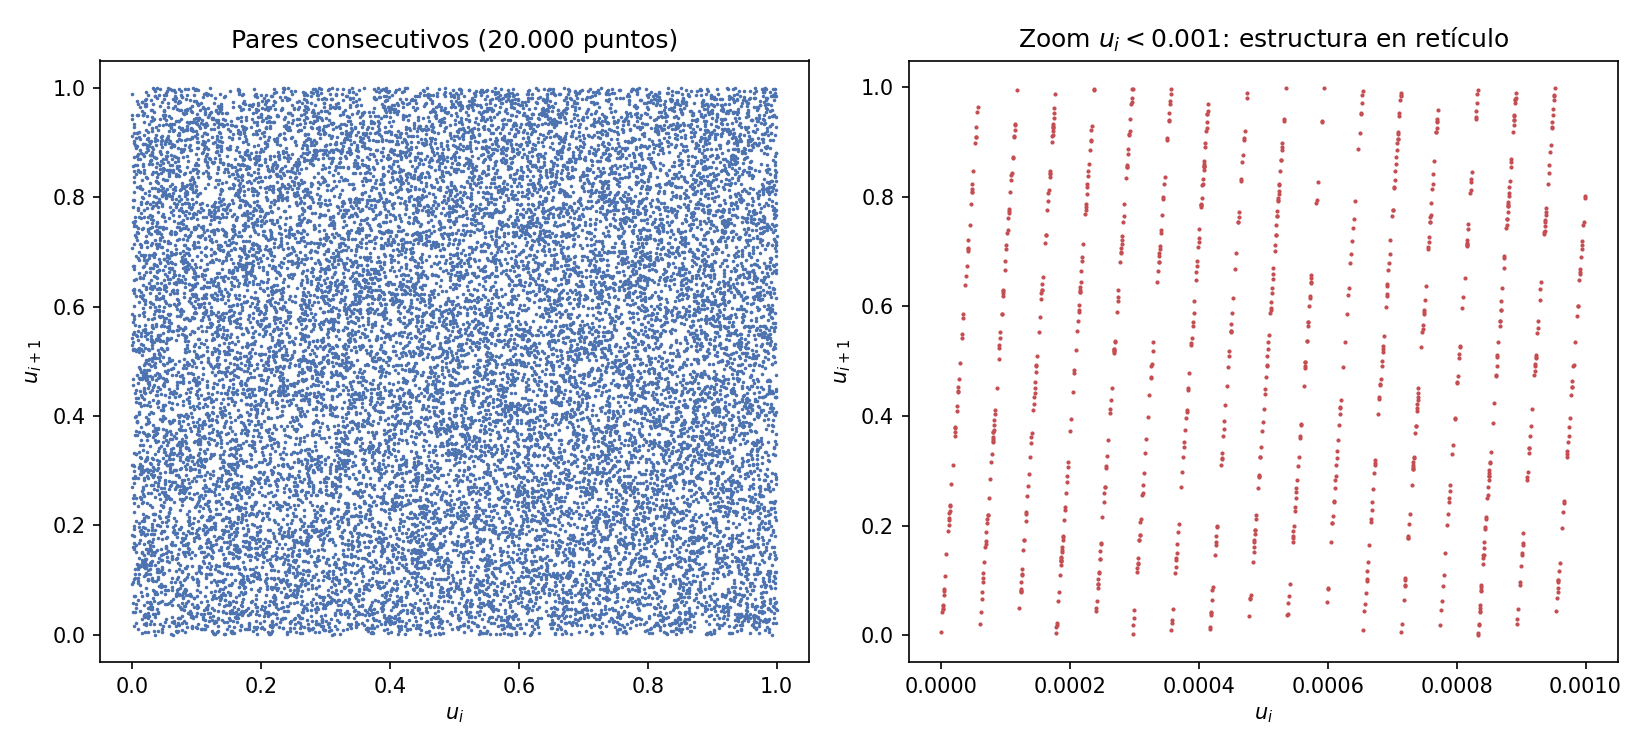
\includegraphics[width=\linewidth]{../figuras/pares.png}
\caption{Pares consecutivos $(u_i,u_{i+1})$ (semilla 12345). Izquierda: 20\,000 puntos. Derecha: ampliación de $u_i<0{,}001$, donde se aprecia el retículo.}
\label{fig:pares}
\end{figure}

%%%%%%%%%%%%%%%%%%%%%%%%%%%%%%%%%%%%%%%%%%%%%%%%%%%%%%%%%%%%%%%%%%%%%%%%
\section{Resultados de la batería Diehard}\label{sec:diehard}

La tabla~\ref{tab:diehard} recoge el p-valor final de cada contraste. Los
contrastes \emph{runs} y \emph{craps} producen dos p-valores cada uno, así que
cada columna suma 18 resultados.

\begin{table}[H]
\centering
\footnotesize
\setlength{\tabcolsep}{4pt}
\begin{tabular}{l ccc c c}
\toprule
 & \multicolumn{3}{c}{u32 (nuestro generador)} & shift & \code{minstd} \\
\cmidrule(lr){2-4}
Contraste & s = 12345 & s = 987654321 & s = 20261130 & s = 12345 & s = 12345 \\
\midrule
birthdays      & 0,665 \PA & 0,351 \PA & 0,528 \PA & 0,505 \PA & 0,974 \PA \\
operm5         & 0,315 \PA & 0,814 \PA & 0,445 \PA & 0,315 \PA & 0,054 \PA \\
rank\_32x32    & 0,000 \FA & 0,000 \FA & 0,000 \FA & 0,000 \FA & 0,996 \WK \\
rank\_6x8      & 0,266 \PA & 0,178 \PA & 0,431 \PA & 0,000 \FA & 0,809 \PA \\
bitstream      & 0,515 \PA & 0,701 \PA & 0,350 \PA & 0,000 \FA & 0,202 \PA \\
opso           & $2\cdot10^{-5}$ \WK & 0,012 \PA & 0,007 \PA & 0,000 \FA & $2\cdot10^{-5}$ \WK \\
oqso           & $6\cdot10^{-7}$ \FA & $1\cdot10^{-6}$ \WK & 0,004 \WK & 0,000 \FA & $9\cdot10^{-4}$ \WK \\
dna            & 0,000 \FA & 0,000 \FA & 0,000 \FA & 0,000 \FA & 0,000 \FA \\
count\_1s\_str & 0,000 \FA & 0,000 \FA & 0,000 \FA & 0,000 \FA & 0,871 \PA \\
count\_1s\_byt & 0,000 \FA & 0,000 \FA & 0,000 \FA & 0,000 \FA & 0,704 \PA \\
parking\_lot   & 0,008 \PA & 0,015 \PA & 0,048 \PA & 0,008 \PA & 0,008 \PA \\
2dsphere       & 0,019 \PA & 0,034 \PA & 0,492 \PA & 0,019 \PA & 0,019 \PA \\
3dsphere       & 0,152 \PA & 0,508 \PA & 0,188 \PA & 0,152 \PA & 0,152 \PA \\
squeeze        & 0,325 \PA & 0,293 \PA & 0,614 \PA & 0,325 \PA & 0,325 \PA \\
runs (1)       & 0,080 \PA & 0,364 \PA & 0,972 \PA & 0,080 \PA & 0,080 \PA \\
runs (2)       & 0,751 \PA & 0,996 \WK & 0,222 \PA & 0,751 \PA & 0,751 \PA \\
craps (victorias) & 0,532 \PA & 0,988 \PA & 0,425 \PA & 0,532 \PA & 0,532 \PA \\
craps (tiradas)   & 0,041 \PA & 0,164 \PA & 0,490 \PA & 0,041 \PA & 0,041 \PA \\
\midrule
\textbf{P / W / F} & 12 / 1 / 5 & 12 / 2 / 4 & 13 / 1 / 4 & 10 / 0 / 8 & 14 / 3 / 1 \\
\bottomrule
\end{tabular}
\caption{p-valores finales de Dieharder (100 repeticiones por contraste). \PA\ = PASSED, \WK\ = WEAK, \FA\ = FAILED. Los valores 0,000 corresponden a $p<10^{-8}$.}
\label{tab:diehard}
\end{table}

\subsection{Análisis}

\textbf{Contrastes superados.} Con todas las semillas y conversiones se
superan los siguientes contrastes: \emph{birthday spacings}, OPERM5,
\emph{parking lot}, distancias mínimas en 2D y 3D, \emph{squeeze},
\emph{runs} y \emph{craps}. Son contrastes \enquote{geométricos} o \enquote{de
aplicación}, que usan los números como valores en $(0,1)$. El único WEAK
(\emph{runs}, semilla 987654321, $p=0{,}996$) es esperable: con 18 resultados
por columna, la probabilidad de que al menos uno caiga en la zona WEAK por puro
azar es $1-0{,}99^{18}\approx 0{,}17$. No se repite con las otras semillas.

\textbf{Coincidencia con \code{minstd}.} Desde \emph{parking lot} hasta
\emph{craps}, los p-valores de nuestro generador (u32 y shift, semilla 12345)
coinciden con los de \code{minstd} hasta el último decimal. Esos contrastes
trabajan con $w_i/2^{32}\approx u_i$, de modo que la coincidencia exacta solo
es posible si la secuencia es idéntica. Así se valida la implementación.

\textbf{Fallos de los contrastes a nivel de bit.} Los contrastes de rango
binario, \emph{bitstream}, OPSO, OQSO, DNA y \emph{count-the-1s} analizan bits
concretos de cada palabra de 32 bits. Sus fallos se explican por la conversión
de 31 a 32 bits:
\begin{itemize}
  \item Con \textbf{shift}, el bit menos significativo vale siempre 0. Todos
        los contrastes a nivel de bit fallan (8 FAILED).
  \item Con \textbf{u32}, como $2^{32}/m = 2 + 2/m$, se cumple
        $w_i = 2x_i + \lfloor 2x_i/m \rfloor$. Es decir, \emph{el bit~0 de
        $w_i$ es siempre igual al bit~31}. Se ha comprobado numéricamente en
        200\,000 valores consecutivos, sin ninguna excepción. Por eso dos columnas
        de cada matriz binaria $32\times32$ son idénticas, su rango nunca puede
        ser 32 y el contraste \emph{rank\_32x32} falla siempre. Los contrastes
        \emph{count-the-1s}, que cuentan unos por byte, también detectan la
        redundancia.
  \item El \code{minstd} interno compone las palabras con los 31 bits válidos,
        y por eso supera \emph{count-the-1s} y queda en WEAK en
        \emph{rank\_32x32}.
\end{itemize}

\textbf{Debilidad propia del generador.} Incluso con el tratamiento correcto de
los 31 bits (columna \code{minstd}), el contraste \textbf{DNA falla} y OPSO y
OQSO dan WEAK. Estos contrastes cuentan \enquote{palabras} solapadas formadas
por pocos bits de números consecutivos. Detectan así la estructura en retículo
de la figura~\ref{fig:pares} y las correlaciones entre bits de números
sucesivos. El resultado concuerda con la literatura: el estándar mínimo es un
generador de calidad aceptable para simulaciones modestas, pero no supera las
baterías modernas~\cite{lecuyer}. Además, su periodo ($\approx2{,}1\cdot10^9$)
es comparable al número de valores que consume Dieharder.

%%%%%%%%%%%%%%%%%%%%%%%%%%%%%%%%%%%%%%%%%%%%%%%%%%%%%%%%%%%%%%%%%%%%%%%%
\section{Explicación de tres contrastes Diehard}\label{sec:tres}

\subsection{Birthday spacings (espaciado de cumpleaños)}

Se eligen $m=512$ \enquote{cumpleaños} en un \enquote{año} de $n=2^{24}$ días.
Cada cumpleaños se obtiene de 24 bits de un número aleatorio. Se ordenan, se
calculan los espaciados entre cumpleaños consecutivos y se cuenta $J$, el número
de valores de espaciado que aparecen repetidos. Bajo $H_0$, $J$ sigue
aproximadamente una distribución de Poisson de parámetro
$\lambda = m^3/(4n) = 2$. El experimento se repite y la frecuencia observada de
$J$ se compara con la Poisson(2) mediante un contraste $\chi^2$. Los
generadores congruenciales con retículo grosero producen demasiados espaciados
repetidos y suelen fallarlo. El generador estudiado lo supera en todas las
configuraciones ($p$ entre 0,35 y 0,97).

\subsection{Parking lot (aparcamiento)}

En un cuadrado de lado 100 se intenta \enquote{aparcar} sucesivamente coches
(círculos de radio 1) en posiciones $(100u_i, 100u_{i+1})$. Un intento falla si
el coche choca con alguno ya aparcado. Tras 12\,000 intentos se cuenta el número
$k$ de coches aparcados con éxito. Por simulación con generadores fiables se
sabe que, bajo $H_0$, $k \approx N(3523;\, 21{,}9)$. Se tipifica
$z=(k-3523)/21{,}9$, se repite el experimento y se contrasta mediante
Kolmogorov--Smirnov que los $z$ siguen una $N(0,1)$. Detecta dependencias entre
coordenadas consecutivas: si los puntos del plano no se reparten bien, caben más
o menos coches de lo esperado. El generador lo supera ($p$ entre 0,008 y 0,048).

\subsection{Craps (juego de dados)}

Se juegan 200\,000 partidas de \emph{craps}, obteniendo cada dado como
$\lfloor 6u \rfloor + 1$. En la primera tirada se gana con 7 u 11 y se pierde con
2, 3 o 12. Con cualquier otro resultado (el \enquote{punto}) se sigue tirando
hasta repetirlo (se gana) o sacar un 7 (se pierde). Se calculan dos estadísticos:
\begin{enumerate}
  \item \textbf{Número de victorias.} La probabilidad teórica de ganar es
        $p=244/495\approx0{,}4929$, de modo que el número de victorias es
        aproximadamente $N\big(np,\, np(1-p)\big)$.
  \item \textbf{Número de tiradas por partida.} Se agrupan las partidas de 21
        tiradas o más y se comparan las frecuencias con las probabilidades
        teóricas mediante un contraste $\chi^2$.
\end{enumerate}
Es un contraste \enquote{de aplicación}: reproduce un uso realista del generador
y es sensible a sesgos en la distribución discreta y a dependencias
secuenciales. El generador supera ambos estadísticos en todas las
configuraciones.

%%%%%%%%%%%%%%%%%%%%%%%%%%%%%%%%%%%%%%%%%%%%%%%%%%%%%%%%%%%%%%%%%%%%%%%%
\section{Conclusiones}\label{sec:conclusiones}

\begin{itemize}
  \item Se ha implementado y validado el generador de IMSL
        $x_{i+1}=16807x_i \bmod (2^{31}-1)$. Su periodo es completo,
        $2^{31}-2$, y coincide exactamente con el valor de control de Park y
        Miller y con el \code{minstd} de Dieharder.
  \item Como fuente de números en $(0,1)$ se comporta bien. Supera los seis
        contrastes clásicos y todos los contrastes Diehard que usan los valores
        en coma flotante: \emph{birthday spacings}, OPERM5, \emph{parking lot},
        esferas, \emph{squeeze}, \emph{runs} y \emph{craps}.
  \item No supera la batería completa. Los fallos a nivel de bit se deben en
        gran parte a que solo tiene 31 bits: con la conversión
        $\lfloor u\cdot2^{32}\rfloor$, el bit 0 replica al bit 31. Sin embargo, el
        fallo de DNA y los resultados WEAK de OPSO y OQSO persisten con el
        tratamiento correcto de los bits. Reflejan la estructura en retículo
        propia de los generadores congruenciales.
  \item Por tanto, el generador es adecuado para simulaciones moderadas que usan
        directamente $u_i$, como las del tema~4. No lo es cuando importan los
        bits individuales, ni para simulaciones que consumen una fracción
        apreciable de su periodo. En esos casos son preferibles generadores
        modernos como Mersenne Twister, PCG o xoshiro.
\end{itemize}

%%%%%%%%%%%%%%%%%%%%%%%%%%%%%%%%%%%%%%%%%%%%%%%%%%%%%%%%%%%%%%%%%%%%%%%%
\appendix
\section{Contenido de la entrega y reproducción}

\begin{itemize}
  \item \code{lcg.c}: generador (modos \code{check}, \code{txt} y \code{raw}).
        Se compila con \code{gcc -O2 -o lcg lcg.c}.
  \item \code{lcg}: ejecutable para Linux x86-64.
  \item \code{run_dieharder.sh}: ejecuta la batería completa y guarda los
        resultados en \code{resultados/}. Necesita Dieharder
        (\code{apt install dieharder}).
  \item \code{contrastes_clasicos.py}: contrastes clásicos y figuras
        (\code{python contrastes_clasicos.py 12345 1000000}).
  \item \code{resultados/}: salidas en bruto de Dieharder y de los contrastes
        clásicos.
\end{itemize}
La muestra no se incluye por su tamaño, pero se regenera de forma determinista
a partir de la semilla.

%%%%%%%%%%%%%%%%%%%%%%%%%%%%%%%%%%%%%%%%%%%%%%%%%%%%%%%%%%%%%%%%%%%%%%%%
\begin{thebibliography}{9}
\bibitem{riosinsua} D. Ríos Insua, S. Ríos Insua, J. Martín y A. Jiménez,
  \emph{Simulación: Métodos y Aplicaciones}, 2.ª ed. Madrid: RA-MA, 2008.
\bibitem{parkmiller} S. K. Park y K. W. Miller, \enquote{Random number
  generators: good ones are hard to find}, \emph{Communications of the ACM},
  vol.~31, n.º~10, pp.~1192--1201, 1988.
\bibitem{diehard} G. Marsaglia, \enquote{The Marsaglia Random Number CDROM
  including the Diehard Battery of Tests of Randomness}, Florida State
  University, 1995.
\bibitem{dieharder} R. G. Brown, D. Eddelbuettel y D. Bauer,
  \enquote{Dieharder: A Random Number Test Suite}, versión 3.31.1. [En línea].
  Disponible: \url{https://webhome.phy.duke.edu/~rgb/General/dieharder.php}
\bibitem{lecuyer} P. L'Ecuyer y R. Simard, \enquote{TestU01: A C library for
  empirical testing of random number generators}, \emph{ACM Transactions on
  Mathematical Software}, vol.~33, n.º~4, art.~22, 2007.
\bibitem{knuth} D. E. Knuth, \emph{The Art of Computer Programming, Vol.~2:
  Seminumerical Algorithms}, 3.ª ed. Addison-Wesley, 1997.
\end{thebibliography}

\end{document}
